\documentclass[11pt]{beamer}
\usepackage[utf8]{inputenc}
\usepackage[spanish]{babel}
%\usepackage{amsmath}
%\usepackage{amsfonts}
%\usepackage{amssymb}
%\usepackage{graphicx}
\usepackage{subfigure} % subfiguras
\usepackage{ragged2e}
%\usepackage{hyperref}
\usepackage{float}
\usepackage{url}
\usepackage{listings}
%\usepackage{xcolor}
\usepackage{algorithm,algorithmic}

\usepackage{mathtools}
\DeclarePairedDelimiter\ceil{\lceil}{\rceil}
\DeclarePairedDelimiter\floor{\lfloor}{\rfloor}

\usepackage{color}
\definecolor{lightgray}{rgb}{.9,.9,.9}
\definecolor{darkgray}{rgb}{.4,.4,.4}
\definecolor{purple}{rgb}{0.65, 0.12, 0.82}

\lstdefinelanguage{JavaScript}{
  keywords={typeof, new, true, false, catch, function, return, null, catch, switch, var, if, in, while, do, else, case, break},
  keywordstyle=\color{blue}\bfseries,
  ndkeywords={class, export, boolean, throw, implements, import, this},
  ndkeywordstyle=\color{darkgray}\bfseries,
  identifierstyle=\color{black},
  sensitive=false,
  comment=[l]{//},
  morecomment=[s]{/*}{*/},
  commentstyle=\color{purple}\ttfamily,
  stringstyle=\color{red}\ttfamily,
  morestring=[b]',
  morestring=[b]"
}

\lstset{
   language=JavaScript,
   backgroundcolor=\color{lightgray},
   extendedchars=true,
   basicstyle=\tiny\ttfamily,
   %basicstyle=\footnotesize\ttfamily,
   showstringspaces=false,
   showspaces=false,
   numbers=left,
   numberstyle=\footnotesize,
   numbersep=4pt,
   tabsize=1,
   breaklines=true,
   showtabs=false,
   captionpos=b
}

\usetheme{Madrid}

%\usepackage{natbib}
\usepackage{bibentry}
\usepackage{graphicx} % Allows including images
\usepackage{booktabs} % Allows the use of \toprule, 

\setbeamertemplate{bibliography item}{\insertbiblabel}

\newcommand{\celda}[1]{
	\begin{minipage}{2.5cm}
		\vspace{5mm}
		#1
		\vspace{5mm}
	\end{minipage}
}

\author[Abarca, Apari, Suca, Vargas] % (optional)
{J.~P.~Abarca\inst{1} \and C.~T.~Apari\inst{1} \and C.~A.~Suca\inst{1} \and A.~Vargas\inst{1}  }
\title[Grupo9]{Práctica 4}
\date{ 24 de Julio del 2021} 
%\date{\currenttime}
\subtitle{Kd-Tree}
\logo{
\includegraphics[scale=0.16]{unsa.png}}
\institute[UNSA]{
	\inst{1}
		Universidad Nacional de San Agustín. Facultad de Producción y Servicios. \\Escuela Profesional de Ciencias de la Computación\\
		Maestría en Ciencias de la Computación \\ Docente: Mg. Vicente Machaca \\
		\vspace{2mm}
}

\AtBeginSection[]
{
	\begin{frame}<beamer>{Contenido}
		\tableofcontents[currentsection,currentsubsection]
	\end{frame}
}

\begin{document}
	
	\begin{frame}
		\maketitle
	\end{frame}

	\begin{frame}{Contenido}
		\tableofcontents
	\end{frame}
	
    %%%%% ARBOL kdtree
    \section{Kd-Tree}
	\subsection{Build Kd-Tree}
	\begin{frame}{Definición}
			\justifying
			\begin{figure}[H]
				\centering
				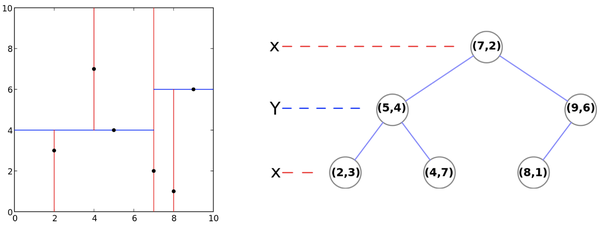
\includegraphics[scale=0.40]{img/kdTree1.png}
				\caption{Construccion del Kd-Tree \cite{Morgan2006}}
				\label{fig:rotacionavl}
			\end{figure}
		\end{frame}
	\begin{frame}{Build Kd-Tree}
			\justifying
			
			\lstinputlisting[language=JavaScript, firstline=53, lastline=78, caption=buildKdtree]{code/kdtree.js}
			
		\end{frame}
	\begin{frame}{Get Height y Generate Dot}
		\justifying
		
		\begin{itemize}
		    \item $get\_Height$, Recursivamente retornamos la altura del nodo izquierdo y derecho, respecto al valor que estamos por recibir tanto de la altura izquierda y derecha 
		    \item $generate\_Dot$, Requerimos solamente imprimir el punto padre que este apuntando a un hijo recursivamente para luego obtener el resultado mediante el graficador Graphviz de Python
		\end{itemize}
		
		
	\end{frame}
	\subsection{Función closestPointBruteForce}
		\begin{frame}{Implementación}
		\justifying
		
		 Directamente comparar la distancia del punto a consultar con  todos  los  puntos  existentes  en  la  lista  completa  generada. 
		
		\lstinputlisting[language=JavaScript, firstline=91, lastline=102, caption=closestPointBruteForce]{code/kdtree.js}
		
	    \end{frame}
		
	\subsection{ Función naiveClosestPoint}
		\begin{frame}{Implementación}
			\justifying
			 Tomando el nodo actual desde el padre hacia los hijos, claramente tiene el mismo comportamiento del que se espera del binary tree \cite{compgeom:2000}.
			 
			\lstinputlisting[language=JavaScript, firstline=104, lastline=121, caption=naiveClosestPoint]{code/kdtree.js}
			
		\end{frame}
	
	\subsection{Evaluación del conjunto de datos}
		\begin{frame}[fragile]\frametitle{Conjunto de datos (1)}
			\justifying
			\begin{verbatim}
			    var data = [
                [40 ,70] ,
                [70 ,130] ,
                [90 ,40] ,
                [110 , 100] ,
                [140 ,110] ,
                [160 , 100]
                ];
                var point = [140 ,90]; 
            \end{verbatim}
			
		\end{frame}
		
		\begin{frame}{Conjunto de datos (1)}
			\justifying
		    
		    \begin{figure}[H]
				\centering
				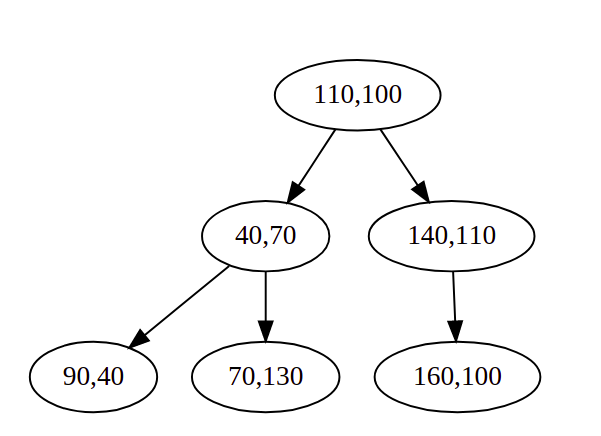
\includegraphics[scale=0.40]{img/query1.png}
				\caption{Resultado en GraphViz}
				\label{fig:graphviz1}
			\end{figure}
			
		\end{frame}
		
		\begin{frame}[fragile]\frametitle{Conjunto de datos (2)}
			\justifying
			\begin{verbatim}
		        var data = [
                [40 ,70] ,
                [70 ,130] ,
                [90 ,40] ,
                [110 , 100] ,
                [140 ,110] ,
                [160 , 100] ,
                [150 , 30]
                ];
                var point = [140 ,90]; 
		    \end{verbatim}  
		    
			
		\end{frame}
		
		\begin{frame}{Conjunto de datos (2)}
			\justifying
		    
		    \begin{figure}[H]
				\centering
				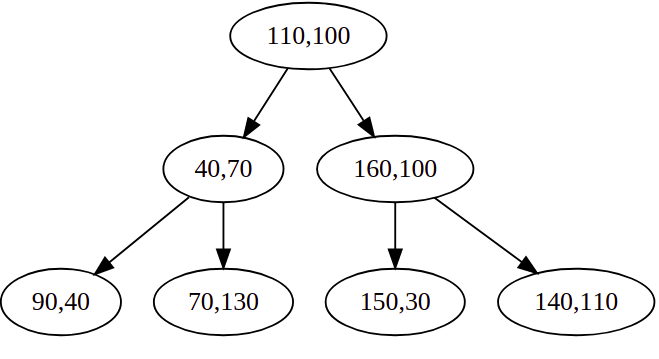
\includegraphics[scale=0.40]{img/query3.png}
				\caption{Resultado en GraphViz}
				\label{fig:graphviz2}
			\end{figure}
			
		\end{frame}
		
		
		
	%%%% Busqueda
	\section{Algoritmos de búsqueda del Kd-Tree}
	    \subsection{Función closest point}
		\begin{frame}{Implementación}
			\justifying
			
			\lstinputlisting[language=JavaScript, firstline=123, lastline=146, caption=closestPoint]{code/kdtree.js}
			
		\end{frame}
		
		\subsection{ Función KNN}
		\begin{frame}{Implementación}
		
			\justifying
			\lstinputlisting[language=JavaScript, firstline=160, lastline=180, caption=KNN1]{code/kdtree.js}
	
			
		\end{frame}
		
		\begin{frame}{Implementación}
			\justifying
		
			\lstinputlisting[language=JavaScript, firstline=181, lastline=198, caption=KNN2]{code/kdtree.js}
			
		\end{frame}
		
		\begin{frame}{Revisión (1)}
			\justifying
			\begin{figure}[H]
				\centering
				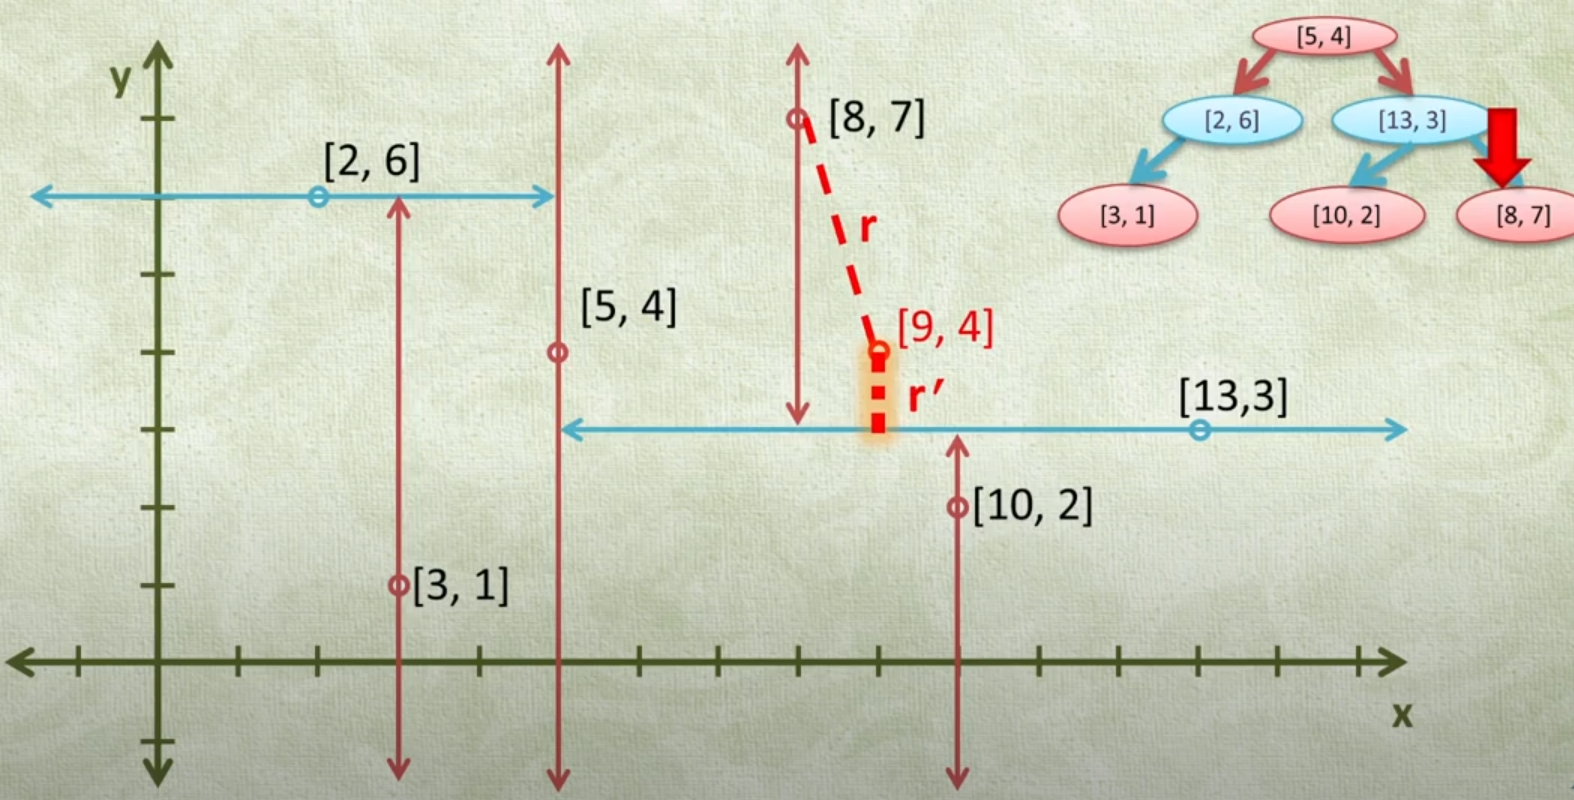
\includegraphics[scale=0.25]{img/knn6.PNG}
				\caption{Punto de revisión}
				\label{fig:knn1}
			\end{figure}
		\end{frame}
		
		\begin{frame}{Revisión (2)}
			\justifying
			\begin{figure}[H]
				\centering
				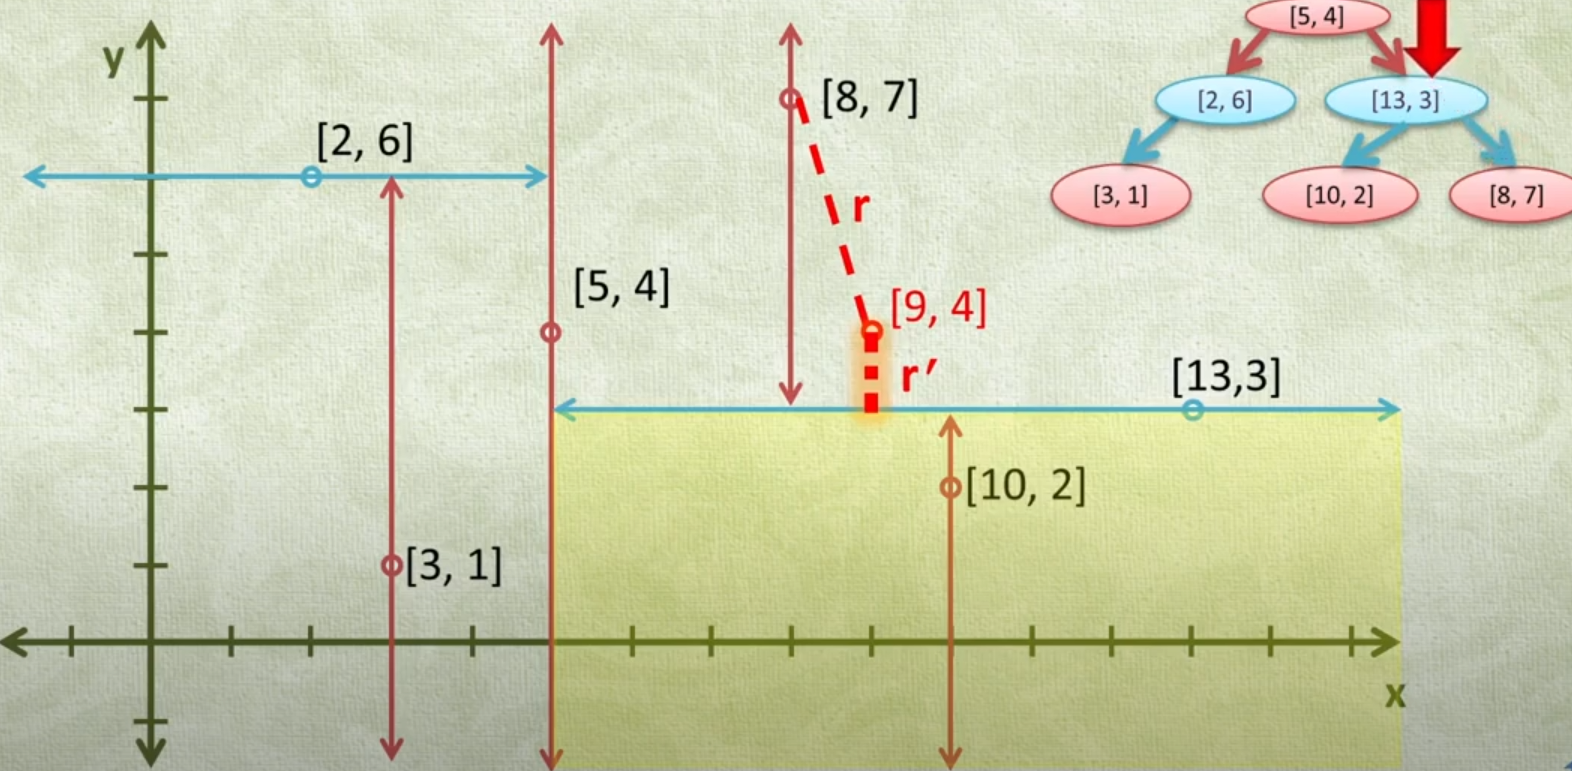
\includegraphics[scale=0.25]{img/knn7.PNG}
				\caption{Punto de revisión}
				\label{fig:knn2}
			\end{figure}
		\end{frame}
		
	
		
		\subsection{Búsqueda - Range Query}
		\begin{frame}{Función $range\_query\_circle$ del KD-Tree}
			\justifying
			\begin{figure}[H]
				\centering
				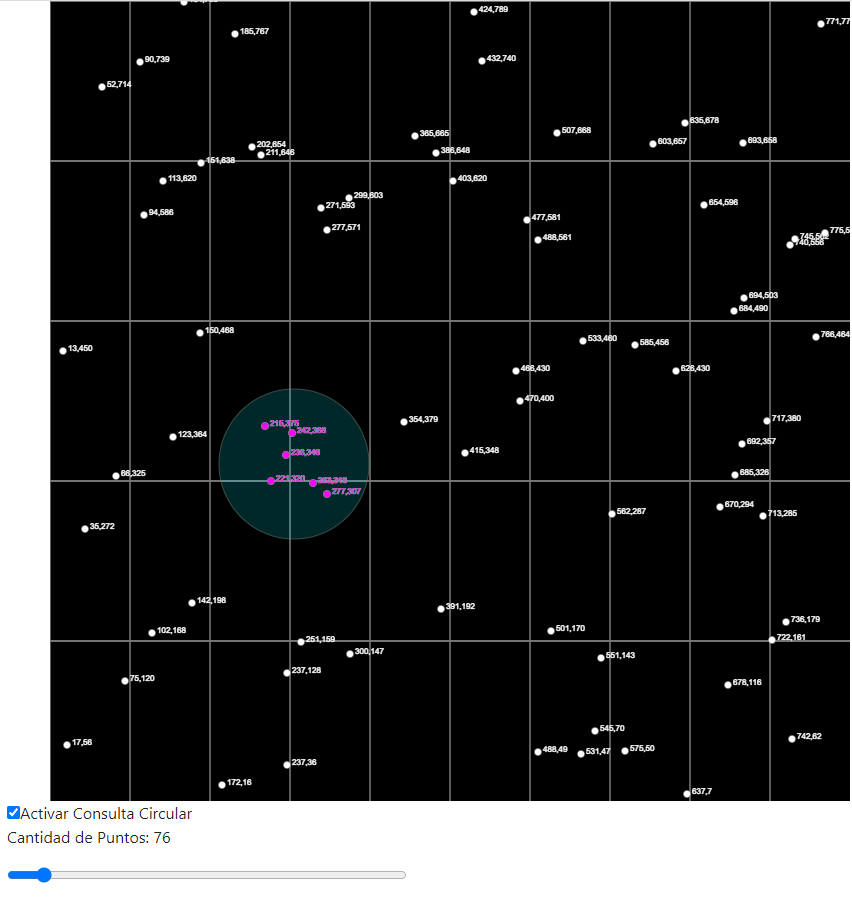
\includegraphics[scale=0.25]{img/circular1.png}
				\caption{Consulta Circular}
				\label{fig:rangeQueryCircle}
			\end{figure}
		\end{frame}
		
		\begin{frame}{Función $range\_query\_rect$ del KD-Tree}
			\justifying
			\begin{figure}[H]
				\centering
				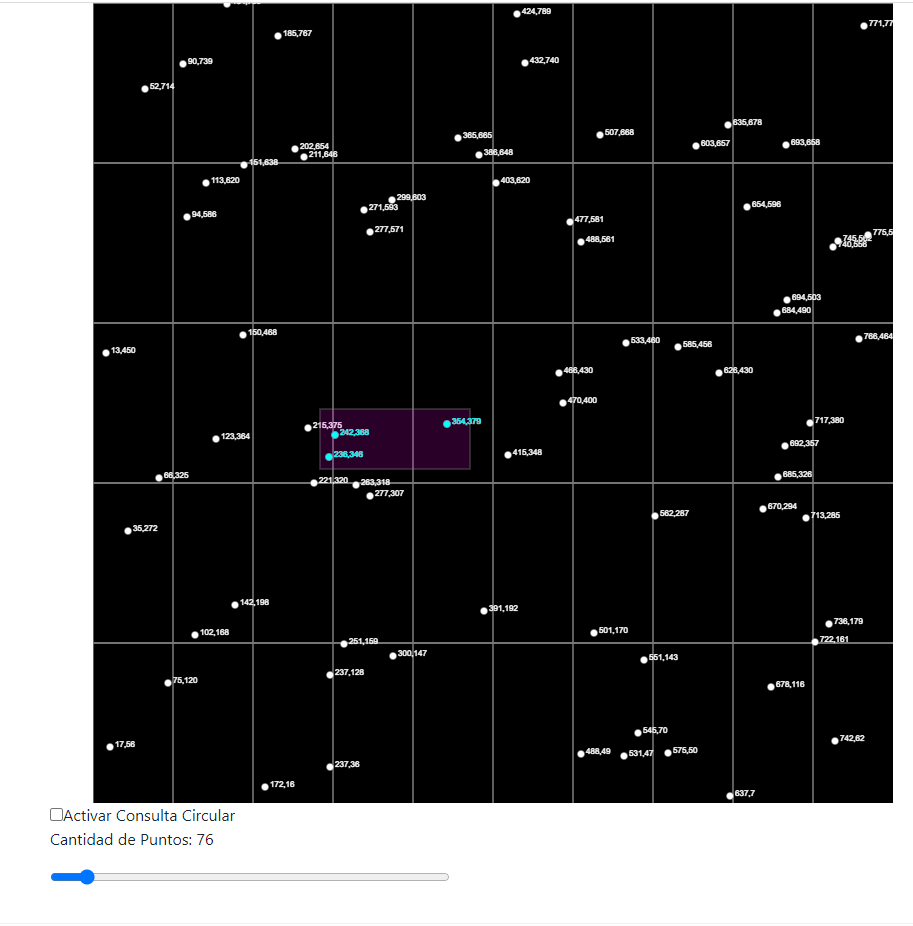
\includegraphics[scale=0.25]{img/rectangular1.png}
				\caption{Consulta Rectangular}
				\label{fig:rangeQueryRect}
			\end{figure}
		\end{frame}
		
		\begin{frame}{}
		    \centering
		    
		    {
		        \Large
		        GRACIAS
		    }
		    
		    \begin{figure}[H]
				\centering
				
\includegraphics[scale=0.1]{img/qr_repositorio.png}
				
				\label{fig:qr_repositorio}
			\end{figure}
			
			Repositorio: \url{https://github.com/jabarcamu/EDA_Practica4}
		    
		\end{frame}

%\appendix
\section{Referencias}
%\subsection<presentation>*{Referencias}

% All of the following is optional and typically not needed. 
%\appendix


\begin{frame}[t, allowframebreaks]
    \frametitle{References}
    \bibliographystyle{ieeetr}
    \bibliography{biblio}
\end{frame}



\end{document}